\hypertarget{part-1-design-5}{
\section{Part 1, design 5}\label{part-1-design-5}}

\begin{figure}[ht]
  \centering
  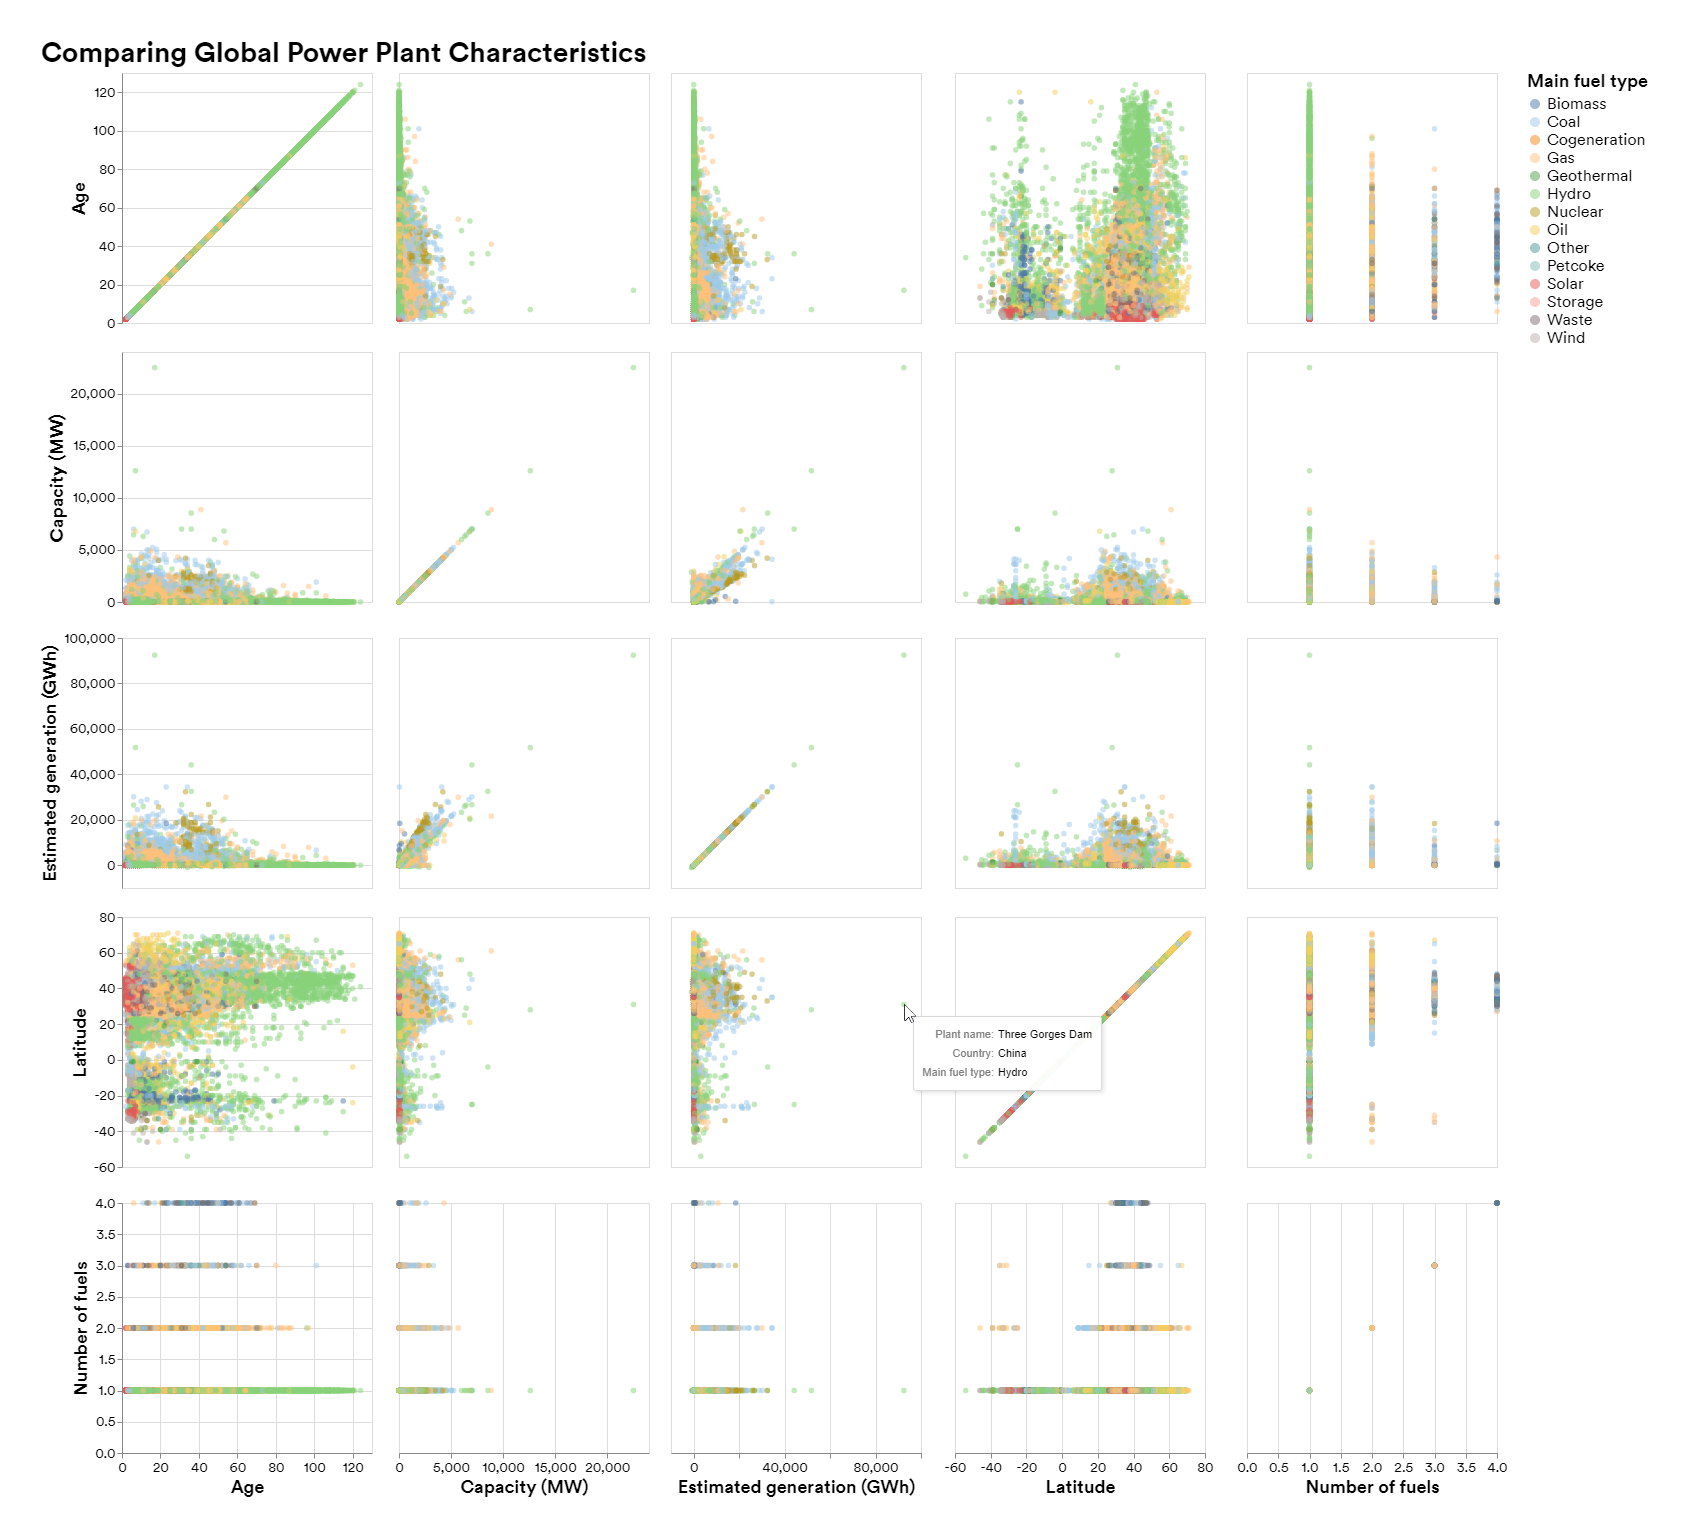
\includegraphics[width=\textwidth]{../img/design5}
  \caption{Comparing global power plant characteristics (Design 5)}
\end{figure}

\hypertarget{description}{
\subsubsection{Description}\label{description}}

\begin{description}
\item[Visual Design Type:]
Scatter plot matrix (SPLOM)
\item[Name of Tool:]
Altair
\item[Country:]
Worldwide
\item[Year:]
2014

\item[Visual Mappings:]
% each of the visual design mappings; include the data apping information about colour, shape, size, position (x/y axes), and any other visual mappings 
\begin{itemize}
  \item \textbf{Attributes}: List of five quantitative attributes for each power plant are compared in every combination to indicate correlation, trends, and outliers.
  \item \textbf{Hue}: Power plant main fuel type.
  \item \textbf{Tooltip}: Tooltips are used to offer detail-on-demand to the user, showing individual plant names and locations.
\end{itemize}

\item[Unique Observation:]
% things we can learn from the visualisation e.g. from this vis we can see this pattern
Correlation between fields is made apparent using this chart, where we can see that there is a distinct lack of power plants located near the equator, and what is there have been constructed recently. The northern hemisphere generates more electricity in general, however global plant capacity can be seen to be proportional to power generated as the two rows appear very similar.

From this perspective, we can also spot the Three Gorges Dam as an obvious outlier to most of our plots with its extremely high capacity and generation. The dam is shown to operate on three fuel types in total and it follows the trend that power plants with more fuel types tend to have greater capacities.

\item[Data Preparation:]
% any modifications to the original data that had to be performed to generate your beautiful image
From the provided GPPD data set, fields were combined and derived to form five key attributes which represent each power plant in the data set. These attributes were then used to sequentially generate charts and populate the SPLOM.

\end{description}

% Describe the insight that your visualizations provide. What can we learn from
% your visualizations? How are they better than a standard line, pie, or bar
% chart?